\documentclass[10pt,a4paper]{report}
\usepackage{color}
\usepackage{xcolor}

% good colors for graphics as in matlab higher versions
\definecolor{bluemat}{rgb}{0, 0.4470 ,0.7410}
\definecolor{redmat}{rgb}{0.8500, 0.3250, 0.0980}
\definecolor{yellowmat}{rgb}{0.9290, 0.6940, 0.1250}
\definecolor{greenmat}{rgb}{0.4660, 0.6740, 0.1880}

\usepackage{tikz}
\usetikzlibrary{arrows,calc}
\usetikzlibrary{arrows.meta}
\begin{document}
\begin{figure}
	\centering
	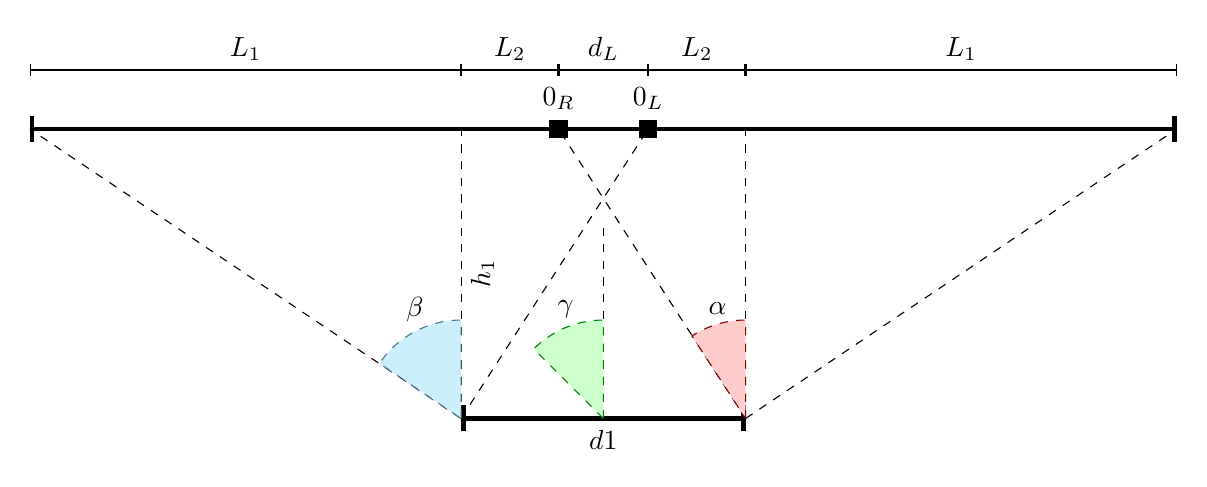
\begin{tikzpicture}[scale=2.5]
	\pgfmathsetmacro{\hOne}{1.47};
	\pgfmathsetmacro{\dOne}{1.445};
	\pgfmathsetmacro{\dL}{0.455};
	\pgfmathsetmacro{\maxR}{2.19};
	\pgfmathsetmacro{\maxL}{\maxR};
	\pgfmathsetmacro{\maxRange}{\maxR+\maxL+\dL};
	\pgfmathsetmacro{\lOne}{0.5*(\maxRange-\dL)};
	\pgfmathsetmacro{\lTwo}{0.5*(\dOne-\dL)};
		
	\coordinate (origin) at (0, 0);
	\coordinate (A) at (-\dOne/2, 0);
	\coordinate (B) at (\dOne/2, 0);
	\coordinate (C) at (-\dOne/2, \hOne);
	\coordinate (D) at (\dOne/2, \hOne);
	\coordinate (E) at (-\dOne/2 - \lOne, \hOne);
	\coordinate (F) at (\dOne/2 + \lOne, \hOne);
	\coordinate (zeroR) at (-\dL/2,\hOne);
	\coordinate (zeroL) at (+\dL/2,\hOne);
	
	
	\draw [Bar-Bar , ultra thick] (A)--(0,0) -- (B) node[align=center, below] at (origin) {$d1$};
	\draw [dashed] (A) -- (C) node[below, midway, rotate=90] {$h_1$};
	\draw [dashed] (B) -- (D);
	\draw [dashed] (origin) -- ++(0, 1);
	\draw [Bar-Bar,ultra thick] (E)--(F);
	% add angles swipes lines
	\draw [dashed] (A)--(E);
	\draw [dashed] (A)--(zeroL);
	\draw [dashed] (B)--(F);
	\draw [dashed] (B)--(zeroR);
	
	% add zeroR and zeroL nodes
	\node[mark=square, fill, label=above:$0_R$] at (zeroR) {};
	\node[mark=square, fill, label=above:$0_L$] at (zeroL) {};
	
	% add arcs of angles
	\filldraw[fill=green!20,draw=green!50!black, dashed] (0,0) -- (0mm,5mm) arc (90:45+90:5mm) node[midway, above]{$\gamma$}-- (0,0);
	
	\filldraw[fill=cyan!20,draw=cyan!50!black, dashed] (A)--($(A)+(0mm,5mm)$) arc (90:56+90:5mm) node[midway, above]{$\beta$} -- (A);
	
	\filldraw[fill=red!20,draw=red!50!black, dashed] (B)--($(B)+(0mm,5mm)$) arc (90:33+90:5mm) node[midway, above]{$\alpha$}--(B);
	
	% add anotations
	\draw [Bar-Bar] (-\dOne/2,\hOne+0.3) -- (-\dL/2,\hOne+0.3) node[align=center, above, midway] {$L_2$};
	\draw [Bar-Bar] (-\dL/2,\hOne+0.3) -- (\dL/2,\hOne+0.3) node[align=center, above, midway] {$d_L$};
	\draw [Bar-Bar] (+\dL/2,\hOne+0.3) -- (\dOne/2,\hOne+0.3) node[align=center, above, midway] {$L_2$};
	\draw [Bar-Bar] (\dOne/2,\hOne+0.3) -- (\dOne/2 + \lOne, \hOne+0.3) node[align=center, above, midway] {$L_1$};
	\draw [Bar-Bar] (-\dOne/2,\hOne+0.3) -- (-\dOne/2 - \lOne, \hOne+0.3) node[align=center, above, midway] {$L_1$};
	\end{tikzpicture}
\end{figure}
\end{document}